\documentclass[main]{subfiles}


\title[AutoML: Introduction]{Learning to Hyperparameter-Optimize}
\subtitle{Can we learn how to HPO with sufficient data?}
\author[Marius Lindauer]{Marius Lindauer}
\date{}

\titlebackground*{images/AutoML_Agentic}

%\institute{}
%\date{}

\begin{document}
	
	\maketitle
	

%----------------------------------------------------------------------
\begin{frame}{Motivation: The Need for Universal HPO}
    \begin{itemize}
        \item \textbf{Problem:} Traditional HPO methods (e.g., Gaussian Processes) struggle to transfer knowledge across tasks with \textit{different} configuration spaces or hyperparameters.
        \item \textbf{Opportunity:} Massive (proprietary) amounts of ``in-the-wild'' tuning data exist, but remain underutilized due to data heterogeneity.
        \item \textbf{Proposal:} A Transformer-based framework that learns a universal prior from vast, diverse offline meta-datasets to solve new optimization tasks.
    \end{itemize}
\end{frame}

\begin{frame}{The OptFormer Concept \liturl{Chen et al. 2022}{https://arxiv.org/abs/2205.13320}}
    \begin{itemize}
        \item \textbf{Core Idea:} Treat HPO as a \textit{sequence modeling} problem.
        \item \textbf{Architecture:} Utilizes a Encoder-Decoder transformer architecture.
        \item \textbf{Universal Interface:} 
            \begin{itemize}
                \item Takes unstructured \textbf{metadata} (search space definitions, algorithm descriptions) and optimization \textbf{history} as input.
                \item Outputs probability distributions over next parameters and function values.
            \end{itemize}
        \item \textbf{Dual Capability:} Simultaneously learns a \textit{Policy} (what to try next) and a \textit{Function Prior} (performance prediction).
    \end{itemize}
\end{frame}

\begin{frame}{Data Representation: Tokenizing HPO \liturl{Chen et al. 2022}{https://arxiv.org/abs/2205.13320}}
    To handle diverse search spaces, prior HPO-data are serialized into a single sequence of discrete tokens.
    
    \begin{itemize}
        \item \textbf{Metadata ($m$):} Textual description of the problem (e.g., parameter names, types, constraints) compressed into tokens.
        \item \textbf{History ($\hist$):} Sequence of trials $(\conf_1, \cost(\conf_1), \dots, \conf_T, \cost(\conf_t))$.
        \item \textbf{Quantization:} Numerical values are normalized and quantized into integers (0-1000) to be treated as vocabulary tokens.
        
        \begin{equation}
            \overline{\conf} = \text{int}[\conf_{norm} \cdot Q] \quad \text{where} \quad \conf_{norm} = \frac{\conf - \conf_{min}}{\conf_{max} - \conf_{min}}
        \end{equation}
        
        \item \textbf{Final Sequence:} $\overline{\hist} = [\overline{\conf}_1, \dots, \overline{\conf}_T, *, \overline{\cost(\conf)}, \dots]$.
    \end{itemize}
\end{frame}

\begin{frame}{Data Representation Example \liturl{Chen et al. 2022}{https://arxiv.org/abs/2205.13320}}

\centering
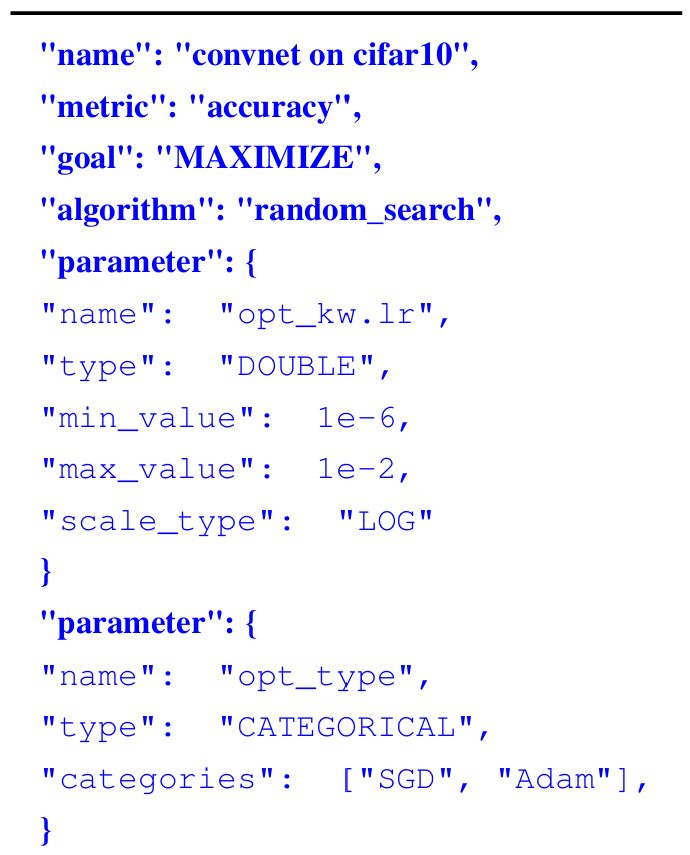
\includegraphics[width=0.3\textwidth]{images/optformer_data1} \qquad
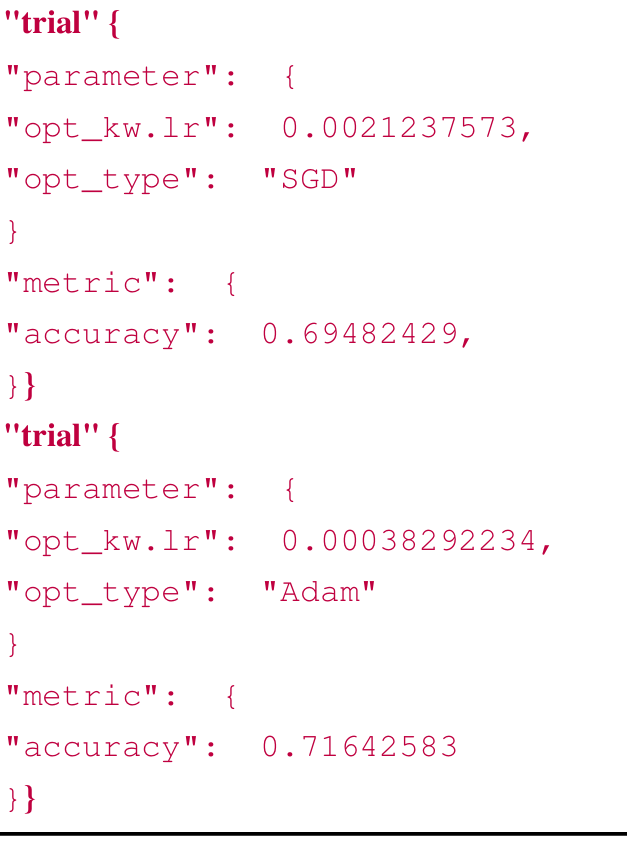
\includegraphics[width=0.3\textwidth]{images/optformer_data2}
    
\end{frame}

% Slide 4: Model Training
\begin{frame}{Training the OptFormer \liturl{Chen et al. 2022}{https://arxiv.org/abs/2205.13320}}
    \begin{itemize}
        \item \textbf{Objective:} Maximize the weighted log-likelihood of the optimization history given metadata and previous history.
        
        \begin{equation}
             \mathcal{L}(\theta) = \sum_{n} w_n \log P_{\theta}(\overline{\hist}^{(n)} \mid m, \overline{\hist}^{(1:n-1)})
        \end{equation}
        
        \item \textbf{Examples of Data Sources:} Trained on a union of RealWorldData (e.g., Google Vizier), HPO-B \liturl{Arango et al. 2021}{https://arxiv.org/abs/2106.06257}, and BBOB (synthetic).
        \item \textbf{Algorithm Imitation:} The model learns to imitate at least 7 distinct HPO algorithms (e.g., Evolutionary, Bayesian, Hill-Climbing) by conditioning on the algorithm name in the metadata.
    \end{itemize}
\end{frame}

\begin{frame}{Inference: The Prior Policy \liturl{Chen et al. 2022}{https://arxiv.org/abs/2205.13320}}
    At inference time, the model acts as a policy $\pi_{prior}$ to generate new hyperparameters.
    
    \begin{itemize}
        \item \textbf{Autoregressive Generation:} Hyperparameters $\conf_t$ are sampled token-by-token from the learned distribution.
        
        \begin{equation}
            \pi_{prior}(\conf_t | m, \hist_{,t-1}) = \prod_{d=1}^{D} p_{\theta}(\conf_t^{(d)} | m, \hist_{,t-1}, \conf_t^{(1:d-1)})
        \end{equation}
        
        \item \textbf{Behavior:} This policy approximates the behavior policy $\pi_b$ seen in training (Behavioral Cloning).
    \end{itemize}
\end{frame}

\begin{frame}{Augmented Policy: Beyond Imitation \liturl{Chen et al. 2022}{https://arxiv.org/abs/2205.13320}}
    To outperform the imitated algorithms, OptFormer uses \textbf{Model-Based Optimization}.
    
    \begin{itemize}
        \item \textbf{Function Prediction:} The model predicts the function value distribution $P_{\theta}(\cost(\conf) | m, \hist_{,t-1}, \conf)$ for any candidate $\conf$.
        \item \textbf{Acquisition Function:} Combining the prior policy with Expected Improvement (EI).
        \item \textbf{Procedure:} 
            \begin{enumerate}
                \item Sample candidates from $\pi_{prior}$.
                \item Select the candidate maximizing $\acq_{EI}$ based on predicted $\surro(\conf)$.
            \end{enumerate}
            
        \begin{equation}
            \conf_{new} \in \text{argmax}_{\conf \sim \pi_{prior}} \mathbb{E}_{P_\theta}[ \max(\cost(\conf) - \cost^*, 0) ]
        \end{equation}
        
        \item[$\leadsto$] OptFormer-EI significantly outperforms baselines and purely imitated policies.
    \end{itemize}
\end{frame}

\begin{frame}{General Takeaways}
    \begin{itemize}
        \item \textbf{Algorithms as Data:} Optimization algorithms can be learned from data rather than hand-engineered.
        \item \textbf{Universality via Text:} Representing search spaces as text allows a single model to adapt to any optimization problem structure.
        \item \textbf{Long-Horizon Transfer:} Transformers can effectively transfer knowledge from offline "wild" data to improve online optimization efficiency.
        \item \textbf{Scalability:} Inference is faster and more scalable than traditional Bayesian Optimization methods for long trial histories.
    \end{itemize}
\end{frame}

\end{document}

